\chapter{Introduction}\label{chap:introduction}

\section{Bugs in Numerical Software}
Numerical software plays a very important role in science, industry, and defense, and failures of numerical software have been reported as the cause of several well-publicized ``disasters" \cite{VuikWeb,Kanewala2014}.  However, automated techniques intended specifically for localizing numerical faults based on execution data have received relatively little attention from researchers, although there has been substantial research on general {\it statistical fault localization} (SFL) techniques (e.g. \cite{Jones2002,Liblit2004,Liu2005}) and on other general automated debugging techniques (see Section 3.6).

%Bugs in the numerical software are often hard to detect because they may not necessarily result in software crashes. It is very difficult to localize the fault by interrupting the execution (e.g. setting a breakpoint) and inspecting the value of intermediate variables, because we lack an oracle that can decide the correctness of intermediate variable values. Testers usually detect failures in numerical programs by checking whether the difference between the program output and expected output exceeds a pre-defined tolerance \cite{commontest}. 

\section{Statistical Fault Localization}
Typical Statistical Fault Localization (SFL) techniques take data characterizing a set of both passing and failing program executions, including PASS/FAIL labels (provided by testers or end users) and recorded profiles of internal program dynamics, and they compute statistical measures of the strength of the association, if any, between the occurrence of software failures and the occurrence of certain runtime events at particular program locations.  These measures are then used to help guide the search for the causes of observed failures, typically by ranking program statements by the strengths of their associations with failures.  When SFL techniques are evaluated they are generally used as the sole source of information about possible fault locations.  However, it seems more realistic to envision them ultimately being used in combination with other sources of information, such as programmer hunches and {\it fault prediction models} \cite{Fenton1999} based on static code properties and project history.  Potentially, SFL techniques provide a relatively inexpensive way to maximize the information obtained by testing.

\section{Causal Statistical Fault Localization}
Causal statistical fault localization (CSFL) aims at localizing faults by estimating {\it average failure-causing effect} (AFCE) for each program element. Average failure-causing effect is defined as the {\it average causal effect} \cite{pearl2000models} of executing a given program element on the occurrence of failures.  

In SFL techniques, the "suspiciousness" of a program element with a statistical measure of the association between coverage of that element and the occurrence of program failures. For example Baah et al showed \cite{baah2010causal} that the Tarantula metric \cite{jones2002visualization}, the Ochiai metric \cite{abreu2007accuracy}, and the F1-measure \cite{manning2008introduction} each embed an estimator of the conditional probability of program failure given that a statement  is covered, which we denote by $P(F|s)$.  We hope these suspiciousness metrics yield good estimates of AFCE in practice. However, Baah et al points out that SFL produce biased estimates of a program element’s AFCE due to confounding bias \cite{baah2010causal}.

\subsection{Confounding Bias}
Confounding Bias is present when the association between a treatment and an outcome is distorted by an extraneous third variable.  For example, Figure \ref{fig2.1} shows a small function that contains a bug in statement $s_3$, which should be $y=x+2$.  Appropriately, $P(F|s_3)=1$.  However, because the faulty statement $s_3$ is always executed before either of the correct statements $s_5$ or $s_8$ is executed, $P(F|s_5)=P(F|s_8)=1$, which suggests misleadingly that $s_5$ and $s_8$ are faulty.

\begin{figure}[htb!]
\vspace{0em}
\begin{center}
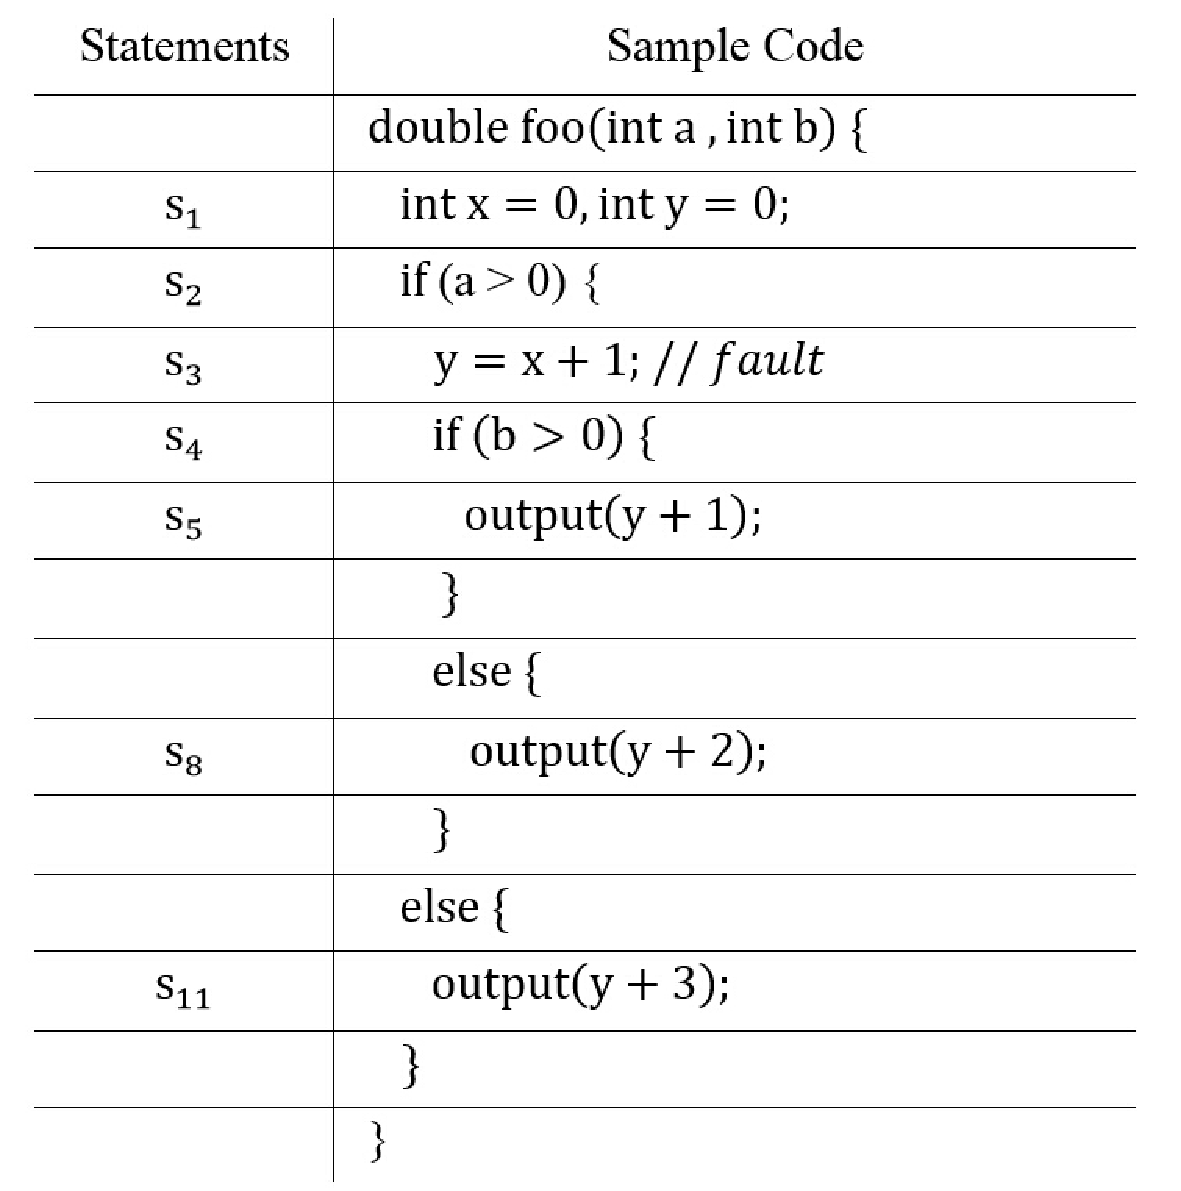
\includegraphics[width=0.6\textwidth]{chapter2_fig1.pdf}
\vspace {0em}\caption{Motivating Example} \label{fig2.1}
\end{center}
\vspace {0em}
\end{figure}
 
This problem, which is an instance of {\it confounding bias} (or just {\it confounding}) \cite{pearl2000models}, is due to the fact that execution of the control dependence region \cite{ball1993s} containing statements $s_3$ and $s_4$ is a {\it common cause} of program failure and of execution of statement $s_5$ or $s_8$.  More generally, confounding of the effect of a ``treatment" variable $T$ on an outcome variable $Y$ is bias due to the presence of a common cause $C$ of $T$ and $Y$.  Confounding bias cannot be eliminated, in general, without considering the causal relationships between the variables under study.  These relationships are typically represented in a {\it causal} DAG \cite{pearl2000models}, which is a directed acyclic graph in which there is an edge $A \rightarrow B$ just in case variable $A$ is a direct cause of variable $B$.  For example, Figure \ref{fig2.2} is a very simple causal graph showing the causal relationships between a treatment $T$, an outcome $Y$, and a confounder $C$.  For SFL, Baah et al \cite{baah2010causal,baah2011mitigating} proposed using a causal DAG derived from the {\it program dependence graph} (PDG) \cite{ferrante1987program}, in which the nodes represent binary coverage indicator variables.

Confounding can be reduced or eliminated by adjusting or controlling for a suitable set of variables during statistical analysis.  A well-known result of Pearl, the {\it Back-Door Adjustment Theorem} \cite{pearl2000models}, states that a set of covariates $\mathbf{X}$ in a causal DAG $G$ is sufficient for confounding adjustment if it ``blocks" all ``backdoor paths" between the treatment $T$ and the outcome $Y$.  A {\it backdoor path} between $T$ and $Y$ is a path with an arrow $T \leftarrow$ entering $T$.  A path is {\it blocked} by $\pmb{X}$ if the path (1) contains a configuration of the form $\rightarrow Z \rightarrow$ or $\leftarrow Z \rightarrow$ such that  $Z \in \mathbf{X}$ or (2) contains a ``collider" $\rightarrow Z \leftarrow$  such that neither $Z$ nor any of its descendants is in $\mathbf{X}$.  For example, in Figure \ref{fig2.2} the path $T \leftarrow C \rightarrow Y$ is a backdoor path, which is blocked by $C$.

\begin{figure}[htb!]
\vspace{0em}
\begin{center}
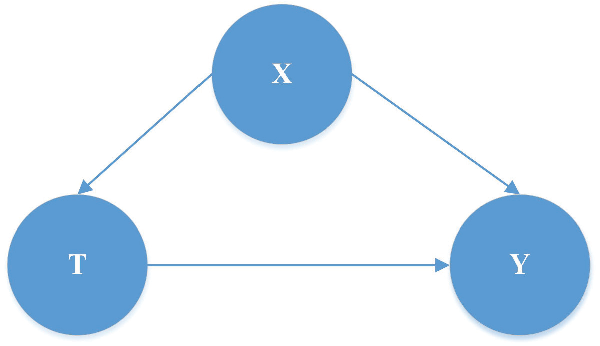
\includegraphics[width=0.6\textwidth]{chapter2_CausalDAG1.pdf}
\vspace {0em}\caption{Causal Diagram of treatment, outcome and confounder} \label{fig2.2}
\end{center}
\vspace {0em}
\end{figure}

\subsection {Baah et al's Coverage-based CSFL}
To adjust (partially) for confounding bias in {\it causal SFL} (CSFL), Baah et al proposed estimating the AFCE of a particular statement $s$ by using a linear regression model of the form
\begin{equation}\label{eq1}
Y=\beta_0+\beta_1T_s+\beta_2C_s+\sigma,
\end{equation}
where $\sigma$ is the treatment (coverage) indicator for $s$ (1: covered, 0: not covered); $C_s$ is a coverage indicator for the {\it forward control dependence predecessor} of $s$ \cite{ball1993s}, which we denote by $pred(s)$; $Y$ is a failure indicator (1: fails; 0: passes); $\beta_0$, $\beta_1$, and $\beta_2$ are coefficients, and $\sigma$ is a random error term.  (Model 1.1) is not applicable to $s$ if $pred(s)$ does not exist.)  Note that the units being "treated" are program executions.  The covariate $C_s$ is used for confounding adjustment in this model because, in the forward control dependence subgraph of the PDG of a structured program, $pred(s)$ blocks all backdoor paths between $T_s$ and $Y$.  (It does not generally block backdoor paths involving data dependences, however.)  The AFCE estimate for $s$ is given by the estimated value $\widehat{\beta_1}$ of the coefficient $\beta_1$ of $T_s$ in model (.11).  This estimate is used as the suspiciousness score of $s$.  Note that an instance of model (1.1) is fitted for each statement.  We shall refer to model (1.1) as Baah et al’s CSFL {\it regression model}.  (Note that Baah et al also proposed another approach to CSFL based on matching instead of regression \cite{baah2011mitigating}, and it does address data dependences.)

\section{Limitations of coverage-based CSFL}
Coverage-based CSFL are subject to two limitations:
\begin{enumerate}
\item In coverage-based CSFL, an important precondition, called "positivity", is often violated. In observational studies, the positivity condition is hold when all conditional probabilities of treatment $\Pr (T = t|X = x) $ are greater than zero. If the positivity condition is violated, the causal effect estimation of coverage-based CSFL may be biased.
\item Coverage-based CSFL does not perform well in localizing faults in the programs that having relatively few conditional branches (e.g. most numerical programs and low-level control systems).
\end{enumerate}  

\section {Contributions}
In this dissertation, our goal is to address the above two limitations of coverage-based CSFL. This is done by: (1) Investigating the effectiveness of coverage-based CSFL under violations of positivity. (2) exploiting localizing faults in numerical software with variable values. 

To address the problem of nonpositivity, we analyze two types of positivity violations: structural violations and random violations and their influences in the Baah et al's causal regression model. We prove that structural violations do occur with Baah et al's causal regression model \cite{baah2010causal} but are not harmful. The random violations of positivity also occur with Baah et al's causal regression model and may result in bias causal effect estimation. To address random violations of positivity, we propose a modification to the way suspiciousness scores are assigned with Baah et al's technique. We also present a probabilistic characterization of Baah et al's estimator, which is more time efficient than Baah et al's estimator to compute the same suspiciousness scores.

To localize faults in numerical programs, we propose two value-based fault localization methods. The first method is NUMFL. We present two variants of NUMF, which use, respectively, the generalized propensity score or the covariate balancing propensity score to control the confounding bias caused by confounding variables, which are variables defined by other faulty expressions.  The  observational dataset of an expression is grouped into several subclasses based on the propensity scores of the data. Within each subclass, NUMFL uses quadratic regression models to estimate the average failure-causing effect of the expression. The second method is based on Bayesian Additve Regression Tree (BART). We use a BART model to approximate the dose-response function (DRF) relating the treatment variable to the output errors. Given a unit in the observational data set, we input it into the fitted BART model, and then increase the value of the treatment variable, but keep the confounding variables unchanged. The causal effect of treatment for that unit is estimated by the change in the output of the BART model. 

Based on our prior work, we also propose FLECS 2.0, a fault localization approach for embedded control software. FLECS 2.0 uses the controller structure and examples of normal behavior in simulation to build structured probabilistic models that compactly encode the dynamic behavior of the system. Given an anomalous behavior sequence, we analyze the values of system state variables to determine which variables are responsible for the behavior. We use the variables obtained in this way together with the dynamic program dependence graph to determine a small set of potential causes (faulty statements) of the behavior, which are then ranked and presented to the developer.

This dissertation makes the following contributions: 
\begin{enumerate}
\item A novel value based approach to SFL for numerical programs
\item An analysis of two types of violations of positivity in casual fault localization
\item The first use of the Bayesian Additive Regression Tree model to estimate failure-causing effects of numerical expressions
\item An improved fault localization approach to fault localization for embedded control systems.
\end{enumerate}

\section{Organization of The Dissertation}

The remainder of the dissertation is organized as follows:

Chapter 2 investigates the performance of Baah et al’s causal regression model for fault localization when the positivity condition is violated.

Chapter 3 presents NUMFL, which is a value based causal inference model for localizing faults in numerical softwares. NUMFL uses generalized propensity scores to control confounding bias.

Chapter 4 presents a new fault localization method, which is based on  the Bayesian Additive Regression Tree model.

Chapter 5 presents FLECS2.0, which is an approach to automatically localize faulty statements in embedded control softwares.

Chapter 6 concludes this dissertation and discusses possible improvements of proposed methods for future work.



